\chapter{Resultados}

\section{Evaluación de nuestra implementación}

En este momento vamos a evaluar debilidades y fortalezas de nuestra implementación de ext2. 

La debilidad obvia, y que no nos importa, es que la implementación no es completa: carece de manejo de permisos de archivos, cosa que no nos importa en DeliriOS.

Además, es mucho más simple que la implementación de ext2 de otros sistemas operativos como Linux, y usa algoritmos mucho menos sofisticados. Sin embargo, no esperaremos que su performance sea mucho peor. Esto lo veremos más adelante.

Una métrica no siempre utilizada al comparar varias implementaciones de una misma especificación es su simplicidad. Aquí sí lo haremos, dado que DeliriOS es un sistema operativo que se concentra en ser minimal, aunque funcional.

Comparemos la cantidad de líneas de código de cada implementación.

\begin{figure}[H]
  \centering
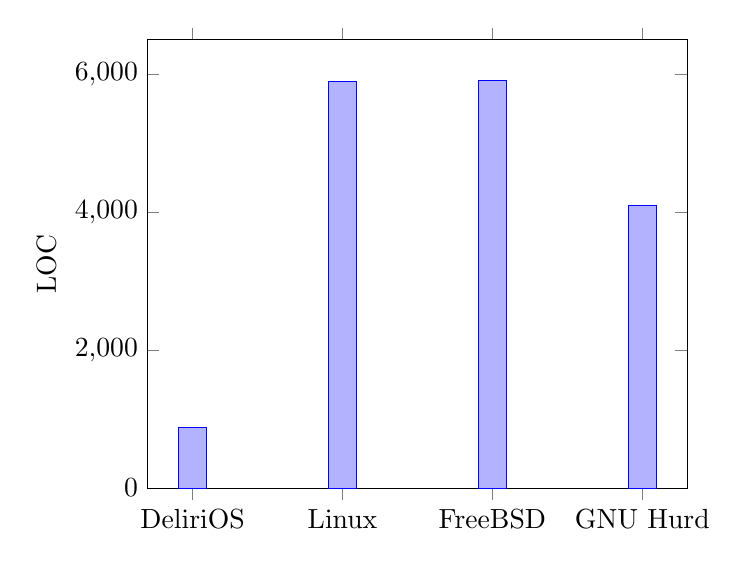
\begin{tikzpicture}
\begin{axis}[
	%x tick label style={/pgf/number format/1000 sep=},
  symbolic x coords={DeliriOS, Linux, FreeBSD, GNU Hurd},
	ylabel=LOC,
  xtick=data,
  ymin=0,
	ybar,
]
\addplot 
	coordinates {
    (DeliriOS,876)
    (Linux,5899)
    (FreeBSD,5910)
    (GNU Hurd,4104)};
\end{axis}
\end{tikzpicture}
\caption{Líneas de código de la implementación de ext2 de cada sistema operativo. El programa \texttt{cloc} fue utilizado para medirlas, dado que cuenta las lineas de código puro, sin contar líneas vacías y de comentarios.}
\end{figure}

\begin{figure}[H]
  \centering
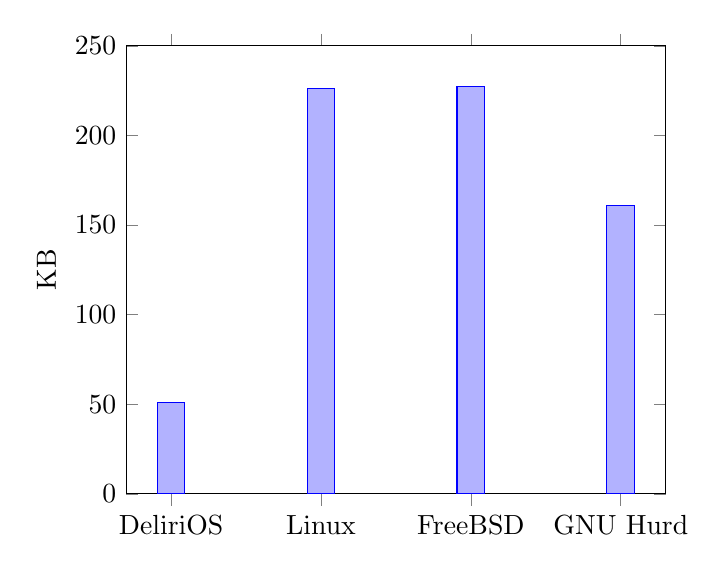
\begin{tikzpicture}
\begin{axis}[
	%x tick label style={/pgf/number format/1000 sep=},
  symbolic x coords={DeliriOS, Linux, FreeBSD, GNU Hurd},
	ylabel=KB,
  xtick=data, 
  ymin=0,
	ybar,
]

%(DeliriOS,52477)
%(Linux,231427)
%(FreeBSD,232832)
%(GNUHurd,164757)};
\addplot 
	coordinates {
    (DeliriOS,51.24)
    (Linux,226.00)
    (FreeBSD,227.37)
    (GNU Hurd,160.89)};
\end{axis}
\end{tikzpicture}
\caption{Tamaño del código fuente de la implementación de ext2 de cada sistema operativo.}
\end{figure}


Como puede verse, la implementación de DeliriOS es realmente simple y corta. Esto es muy bueno, dado que por un lado es más fácil de entender para alguien que se acople al proyecto, y por otro lado permite que el binario de DeliriOS siga siendo diminuto (entra entero en la cache L1 de código de un core de un procesador moderno).



\section{Performance de nuestra implementación}

Para medir la performance de nuestra implementación decidimos compararla con la de Linux.
Tenemos que aclarar que medir este tipo de piezas de software y compararlas es muy difícil por varias razones.
Por ejemplo, como son operaciones dentro de todo muy rápidas, por lo que si las mediciones están mal hechas, el \emph{preemption} del sistema operativo las puede arruinar.

Como DeliriOS sólo soporta ATA PIO por ahora, necesitamos algún ambiente de prueba en el que esto no sea un limitante. Por eso, testeamos sobre una máquina virtual que emulara este tipo de disco.

Las mediciones las tomamos de la siguiente manera: linkeamos los mismos tests que los tests de correctitud por fuera de delirios y los usamos para testear distintas operaciones sobre una imagen de disco.
Tambi\'en realizamos las mismas operaciones con Linux.
Esto ya es un problema, porque el código de DeliriOS va a correr en \emph{userspace}, mientras que el código de Linux va a correr en \emph{kernelspace}.
Veremos cómo corregir esto más adelante, pero primero veamos cómo testeamos. Realizamos 500 repeticiones de cada test, y cada test consistió en lo siguiente.

\begin{itemize}
    \item[create] 36 archivos creados.
    \item[mkdir] 10 directorios creados.
    \item[read] 104000 caract\'eres leídos de 2 archivos.
    \item[remove] 8 archivos borrados.
    \item[write] 104000 caract\'eres escritos en 2 archivos.
\end{itemize}

Todos los tests fueron corridos con el correspondiente flush a disco (fsync en Linux) de tal manera que sean efectivos.

Veamos los resultados.


\begin{figure}[H]
  \centering
  \begin{minipage}[b]{0.49\textwidth}
    \includegraphics[width=\textwidth]{tiempos/create.pdf}
    \caption{}
  \end{minipage}
  \begin{minipage}[b]{0.49\textwidth}
    \includegraphics[width=\textwidth]{tiempos/mkdir.pdf}
    \caption{}
  \end{minipage}
  \hfill
\end{figure}
\begin{figure}[H]
  \centering
  \begin{minipage}[b]{0.49\textwidth}
    \includegraphics[width=\textwidth]{tiempos/read.pdf}
    \caption{}
  \end{minipage}
  \begin{minipage}[b]{0.49\textwidth}
    \includegraphics[width=\textwidth]{tiempos/remove.pdf}
    \caption{}
  \end{minipage}
\end{figure}
\begin{figure}[H]
  \centering
  \includegraphics[width=0.5\textwidth]{tiempos/write.pdf}
  \caption{}
\end{figure}

Sin embargo,...

\begin{figure}[H]
  \centering
  \begin{minipage}[b]{0.49\textwidth}
    \includegraphics[width=\textwidth]{tiempos/create_corregido.pdf}
    \caption{}
  \end{minipage}
  \begin{minipage}[b]{0.49\textwidth}
    \includegraphics[width=\textwidth]{tiempos/mkdir_corregido.pdf}
    \caption{}
  \end{minipage}
\end{figure}
\begin{figure}[H]
  \begin{minipage}[b]{0.49\textwidth}
    \includegraphics[width=\textwidth]{tiempos/read_corregido.pdf}
    \caption{}
  \end{minipage}
  \begin{minipage}[b]{0.49\textwidth}
    \includegraphics[width=\textwidth]{tiempos/remove_corregido.pdf}
    \caption{}
  \end{minipage}
\end{figure}
\begin{figure}[H]
  \centering
  \includegraphics[width=0.5\textwidth]{tiempos/write_corregido.pdf}
  \caption{}
\end{figure}


